\subsection{Create OpenScienceLab Notifications}

\begin{enumerate}
\item Create a new event in your notification calendar\begin{enumerate}
\item The event title corresponds to the notification title
\item Select the time or date range for which you would like to display the notification
\item The remaining notification details are included in the event description\begin{enumerate}
\item Add a \texttt{\textless meta\textgreater } tag\begin{enumerate}
\item Define profiles for which to display notification (profile names may contain spaces)\begin{enumerate}
\item \texttt{profile: profile\_1, profile\_2, profile\_n}\begin{enumerate}
\item \textbf{Note:} comma separated with no spaces
\end{enumerate}
\end{enumerate}


\item Define notification type\begin{enumerate}
\item \texttt{type: info} is blue
\item \texttt{type: warning} is yellow
\item \texttt{type: success} is green
\item \texttt{type: error} is red
\end{enumerate}


\item \textit{Optional} hide notification\begin{enumerate}
\item \texttt{mute: true}
\end{enumerate}
\end{enumerate}


\item Add a \texttt{\textless message\textgreater } tag\begin{enumerate}
\item Add your message body as html\begin{enumerate}
\item Add line breaks\begin{enumerate}
\item \texttt{\textless /br\textgreater }
\end{enumerate}


\item Add links\begin{enumerate}
\item \texttt{\textless a href="https://url.com" target="blank"\textgreater \textless span style="color: blue"\textgreater link\textless /span\textgreater \textless /a\textgreater }\begin{enumerate}
\item \textbf{Note:} You must unlink the URL using the unlink button in the calendar message tool bar for it to work.
\end{enumerate}
\end{enumerate}
\end{enumerate}


\item Turn off text automated formatting\begin{enumerate}
\item Select all the text in the message body
\item Click the remove formatting button in the message toolbar
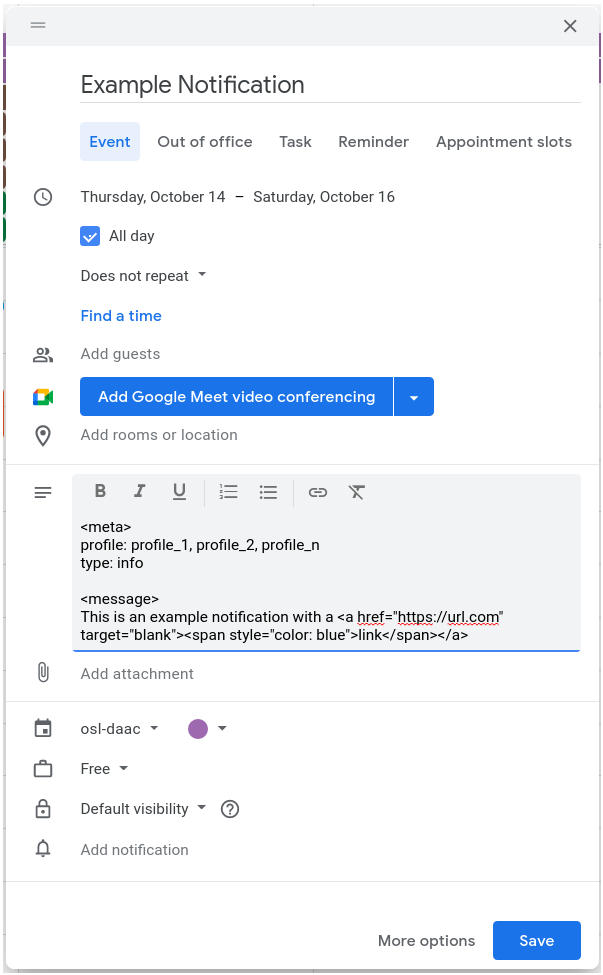
\includegraphics[width=0.7\linewidth]{files/notification-0c08031580ee7d5b2cd20394bd1f7f49.png}
\end{enumerate}
\end{enumerate}
\end{enumerate}
\end{enumerate}
\end{enumerate}